\documentclass[12pt, a4paper]{article}

% ---------------------------------------------------------------------------
% PACOTES
% ---------------------------------------------------------------------------
\usepackage[brazilian]{babel} 
\usepackage[utf8]{inputenc}
\usepackage[T1]{fontenc}
\usepackage{geometry}
\usepackage{graphicx}
\usepackage{hyperref}
\usepackage{listings}
\usepackage{xcolor}
\usepackage{titlesec}
\usepackage{booktabs}
\usepackage{tabularx}
\usepackage{longtable}
\usepackage{array}
\usepackage{indentfirst}
\usepackage{setspace}
\usepackage{fancyhdr}
\usepackage{cite}
\usepackage{amsmath} % CORRIGIDO: Necessário para o \xrightarrow em modelagem.tex
\usepackage{amssymb}
% ---------------------------------------------------------------------------
% CONFIGURAÇÕES DE LAYOUT
% ---------------------------------------------------------------------------
\geometry{
	top=3cm, bottom=2cm,
	left=3cm, right=2cm
}

\setlength{\parindent}{1.25cm}
\setlength{\parskip}{0.2cm}
\onehalfspacing

\hypersetup{
	colorlinks=true,
	linkcolor=blue!70!black,
	urlcolor=blue!70!black,
	citecolor=black
}

% ---------------------------------------------------------------------------
% CONFIGURAÇÃO DOS LISTINGS (Código-Fonte)
% ---------------------------------------------------------------------------
\definecolor{codegray}{rgb}{0.5,0.5,0.5}
\definecolor{codepurple}{rgb}{0.58,0,0.82}
\definecolor{codeblue}{rgb}{0,0.4,0.8}
\definecolor{backcolour}{rgb}{0.97,0.97,0.97}

\lstdefinestyle{javaStyle}{
	backgroundcolor=\color{backcolour},
	commentstyle=\color{codegray},
	keywordstyle=\color{codeblue}\bfseries,
	numberstyle=\tiny\color{codegray},
	stringstyle=\color{codepurple},
	basicstyle=\ttfamily\footnotesize,
	breakatwhitespace=false,
	breaklines=true,
	captionpos=b,
	keepspaces=true,
	numbers=left,
	numbersep=5pt,
	showspaces=false,
	showstringspaces=false,
	showtabs=false,
	tabsize=4,
	frame=single,
	language=Java,
	extendedchars=true, % CORRIGIDO: Melhora suporte a acentuação externa
	literate={á}{{\'a}}1 {ã}{{\~a}}1 {í}{{\'i}}1 {ó}{{\'o}}1 {é}{{\'e}}1 {ç}{{\c{c}}}1 {ú}{{\'u}}1 {ê}{{\^e}}1 {â}{{\^a}}1 {A}{A}1 {&}{{\&}}1 % CORRIGIDO: Escapa o & e acentos dentro do código
}

\lstdefinestyle{sqlStyle}{
	backgroundcolor=\color{backcolour},
	commentstyle=\color{codegray}\itshape,
	keywordstyle=\color{codeblue}\bfseries,
	numberstyle=\tiny\color{codegray},
	basicstyle=\ttfamily\footnotesize,
	breaklines=true,
	frame=single,
	language=SQL,
	extendedchars=true,
	literate={á}{{\'a}}1 {ã}{{\~a}}1 {í}{{\'i}}1 {ó}{{\'o}}1 {é}{{\'e}}1 {ç}{{\c{c}}}1 {ú}{{\'u}}1 {ê}{{\^e}}1 {â}{{\^a}}1 {&}{{\&}}1
}

\lstset{style=javaStyle}

% ---------------------------------------------------------------------------
% CONFIGURAÇÃO DE CABEÇALHO E RODAPÉ
% ---------------------------------------------------------------------------
\pagestyle{fancy}
\fancyhf{}
\rhead{\footnotesize APO2 - Biblioteca MARC21}
\lhead{\footnotesize Documentação Técnica}
\rfoot{\thepage}
\renewcommand{\headrulewidth}{0.4pt}

% ---------------------------------------------------------------------------
% INÍCIO DO DOCUMENTO
% ---------------------------------------------------------------------------
\begin{document}
	
	\pagenumbering{Alph} 
	
	% ---------------------------------------------------------------------------
	% CAPA
	% ---------------------------------------------------------------------------
	\begin{titlepage}
		\centering
		\vspace*{2cm}
		{\LARGE \textbf{CURSO DE ANÁLISE E DESENVOLVIMENTO DE SISTEMAS}\par}
		\vspace{0.5cm}
		{\large Disciplina: Algoritmos e Programação Orientada a Objetos II (APO2)\par}
		\vspace{3cm}
		{\Huge \textbf{Sistema de Gestão de Biblioteca MARC21}\par}
		\vspace{0.5cm}
		{\large Plataforma Jakarta EE --- Apache Tomcat 9.0\par}
		\vspace{2cm}
		{\large
			\textbf{Integrantes:}\par
			\vspace{0.5cm}
			Hálan Sousa, Naiany Sobral, Maria Machado\par
		}
		\vfill
		
	\end{titlepage}
	
	\clearpage
	\pagenumbering{arabic}
	
	% ---------------------------------------------------------------------------
	% SUMÁRIO
	% ---------------------------------------------------------------------------
	\tableofcontents
	\newpage
	
	% ---------------------------------------------------------------------------
	% INCLUSÃO DAS SEÇÕES
	% ---------------------------------------------------------------------------
	\section{Objetivo do Sistema}
	O presente trabalho tem como objetivo o desenvolvimento de um \textbf{Sistema de Gestão de Biblioteca} utilizando a plataforma \textbf{Jakarta EE (Java EE 8)}, com servidor de aplicação \textbf{Apache Tomcat 9.0}, banco de dados \textbf{MySQL 8.0} e interface web construída com \textbf{Bootstrap 5.0} e requisições assíncronas via \textbf{jQuery/AJAX}.

O sistema foi concebido para atender as necessidades operacionais de uma biblioteca de médio porte, contemplando as seguintes funções principais:

\begin{itemize}
    \item \textbf{Catalogação do Acervo Bibliográfico:} Registro de obras físicas com suporte ao padrão internacional \textbf{MARC21} (\textit{Machine-Readable Cataloging}), permitindo a indexação de metadados bibliográficos como título (Tag 245), autor (Tag 100), ISBN (Tag 020) e assuntos (Tag 650), entre outros.
    
    \item \textbf{Controle de Solicitações, Empréstimos e Devoluções:} Gerenciamento do ciclo de vida completo do empréstimo de livros físicos, incluindo solicitação pelo leitor, aprovação ou recusa pelo administrador, registro de retirada, controle de prazos (prazo padrão de 7 dias corridos), registro de devoluções e cálculo automático de multas por atraso.
    
    \item \textbf{Renovação Online:} Permite que leitores autenticados renovem o prazo de seus empréstimos de forma assíncrona, respeitando o limite máximo de renovações configurável pelo administrador.
    
    \item \textbf{Gestão de Usuários e Controle de Acesso (RBAC):} O sistema implementa o padrão de segurança por Controle de Acesso Baseado em Papéis (\textit{Role-Based Access Control}), diferenciando os perfis de \textbf{Administrador} e \textbf{Cliente (Leitor)}.
    
    \item \textbf{Validação de Cadastro por E-mail:} Usuários recém-cadastrados precisam confirmar seu endereço de e-mail através de um link de ativação gerado com token único (\texttt{UUID}), enviado via protocolo \textbf{SMTP} com suporte ao serviço de testes \textbf{Mailtrap}.
    
    \item \textbf{Listas de Leitura Personalizadas:} Leitores podem criar coleções pessoais de livros de interesse, como pastas de favoritos.
    
    \item \textbf{Configurações Operacionais Dinâmicas:} Administradores podem ajustar parâmetros como o valor da multa diária e o limite de renovações diretamente pelo painel administrativo, sem necessidade de intervenção no código.
\end{itemize}

O projeto foi desenvolvido com base no \textbf{Documento de Diretrizes Arquiteturais} elaborado previamente, seguindo os princípios \textbf{SOLID} --- em especial o Princípio da Substituição de Liskov (LSP) na hierarquia de herança do acervo (\texttt{ItemAcervo} $\rightarrow$ \texttt{LivroFisico}, \texttt{EBook}) e o Princípio Aberto/Fechado (OCP) na extensibilidade das classes de persistência (\texttt{BaseDAO}).

A arquitetura segue o padrão \textbf{MVC (Model--View--Controller)}, separando claramente as responsabilidades entre as camadas de modelo (Entidades e DAOs), controle (Servlets HTTP) e visão (páginas JSP com Bootstrap).

	
	\section{Equipe e Funções dos Integrantes}
	A equipe responsável pelo desenvolvimento deste projeto é composta pelos seguintes integrantes:

\begin{table}[h!]
\centering
\caption{Integrantes e participação no projeto}
\label{tab:equipe}
\begin{tabularx}{\textwidth}{|l|X|}
\hline
\textbf{Integrantes} & \textbf{Participação} \\
\hline
Hálan Sousa, Naiany Sobral e Maria Machado &
Todos os integrantes participaram de forma conjunta em todas as etapas do desenvolvimento do projeto, incluindo levantamento de requisitos, modelagem do banco de dados, implementação do back-end e do front-end, integração entre as camadas, testes, documentação e validação das funcionalidades, sem divisão fixa de responsabilidades. \\
\hline
\end{tabularx}
\end{table}


	
	\section{Requisitos do Sistema}
	\subsection{Requisitos Tecnológicos}

O projeto foi desenvolvido atendendo integralmente os seguintes requisitos tecnológicos obrigatórios:

\begin{table}[h!]
	\centering
	\caption{Requisitos tecnológicos e status de atendimento}
	\label{tab:req_tec}
	\begin{tabular}{|p{4.5cm}|p{9.5cm}|c|}
		\hline
		\textbf{Tecnologia} & \textbf{Aplicação no Projeto} & \textbf{Status} \\ \hline
		Jakarta EE / Tomcat 9+ & Servidor de aplicação principal; API de Servlets 4.0 & $\checkmark$ \\ \hline
		MySQL Server 8.0+ & Banco de dados relacional; scripts em \texttt{ddl.sql} e \texttt{dml.sql} & $\checkmark$ \\ \hline
		jQuery & Requisições AJAX, manipulação DOM, máscaras de entrada & $\checkmark$ \\ \hline
		Bootstrap 5.0 & Layout responsivo, componentes visuais, modais & $\checkmark$ \\ \hline
		AJAX & Chamadas assíncronas para todos os endpoints & $\checkmark$ \\ \hline
		Endpoints JSON & Retorno \texttt{application/json} em todos os Servlets & $\checkmark$ \\ \hline
		Testes Postman & Relatório de testes na Seção~\ref{sec:testes_endpoints} & $\checkmark$ \\ \hline
		Servlets como endpoints & Todos os endpoints são Servlets mapeados por anotações \texttt{@WebServlet}; o \texttt{web.xml} define a página inicial & $\checkmark$ \\ \hline
		JSP para views & Todas as páginas são construídas em JSP com JSTL & $\checkmark$ \\ \hline
	\end{tabular}
\end{table}

\subsection{Requisitos Funcionais}

\begin{itemize}
	\item \textbf{RF01} --- Cadastro de Usuário: Permite o auto-cadastro de leitores informando nome, e-mail e senha.
	\item \textbf{RF02} --- Ativação de Conta: Envio de e-mail assíncrono com token exclusivo para validação do cadastro.
	\item \textbf{RF03} --- Autenticação: Sistema de login seguro diferenciando perfis por papéis através de filtros.
	\item \textbf{RF04} --- Recuperação de Senha: Gera uma senha provisória aleatória e envia ao e-mail do usuário ativo.
	\item \textbf{RF05} --- Consulta ao Acervo: Filtros e buscas de livros e e-books por título, autor ou assunto.
	\item \textbf{RF06} --- Detalhes do Item: Visualização completa dos metadados bibliográficos estruturados no padrão MARC21.
	\item \textbf{RF07} --- Solicitação de Empréstimo: Leitores com conta ativa e sem débitos podem solicitar a retirada de livro físico disponível, ficando a solicitação pendente de aprovação administrativa.
	\item \textbf{RF08} --- Renovação Assíncrona: Extensão do prazo de entrega via painel do leitor, respeitando limites operacionais.
	\item \textbf{RF09} --- Listas de Interesse: Criação e gerenciamento de coleções de favoritos de livros físicos pelo leitor.
	\item \textbf{RF10} --- Painel de Controle (Dashboard): Indicadores gráficos e contadores quantitativos específicos para administradores e leitores.
	\item \textbf{RF11} --- Gerenciamento de Acervo: Cadastro, edição e exclusão de livros físicos e e-books, incluindo campos MARC21.
	\item \textbf{RF12} --- Gerenciamento de Usuários: Listagem de usuários, alteração de perfil (admin/leitor) e inativação.
	\item \textbf{RF13} --- Controle de Empréstimos: Aprovação ou recusa de solicitações pelo administrador, registro de devolução e visualização de pendências.
	\item \textbf{RF14} --- Relatório de Inadimplência: Listagem de empréstimos em atraso com cálculo de multa acumulada.
	\item \textbf{RF15} --- Configurações do Sistema: Ajuste de parâmetros operacionais (prazo padrão, valor de multa, limite de renovações).
\end{itemize}

\subsection{Requisitos Não-Funcionais}

\begin{itemize}
	\item \textbf{RNF01 --- Segurança:} Senhas armazenadas com hash SHA-256. Sessões gerenciadas pelo Tomcat com filtro de autenticação em todas as rotas protegidas.
	\item \textbf{RNF02 --- Usabilidade:} Interface responsiva (Bootstrap 5) com feedback imediato ao usuário via mensagens AJAX.
	\item \textbf{RNF03 --- Manutenibilidade:} Arquitetura em camadas (MVC) com padrão DAO e herança (\texttt{BaseDAO}), seguindo os princípios SOLID.
	\item \textbf{RNF04 --- Portabilidade:} Empacotado como \texttt{.war} compatível com qualquer container Servlet 4.0+ (Tomcat 9/10, WildFly, GlassFish).
\end{itemize}

	
	\section{Modelagem do Sistema}
	\subsection{Diagrama de Classes}

O sistema foi projetado seguindo uma hierarquia de herança clara para o acervo bibliográfico. A classe abstrata \texttt{ItemAcervo} define o contrato comum para todos os itens do acervo, sendo estendida pelas classes concretas \texttt{LivroFisico} e \texttt{EBook}.

\begin{figure}[htbp]
	\centering
	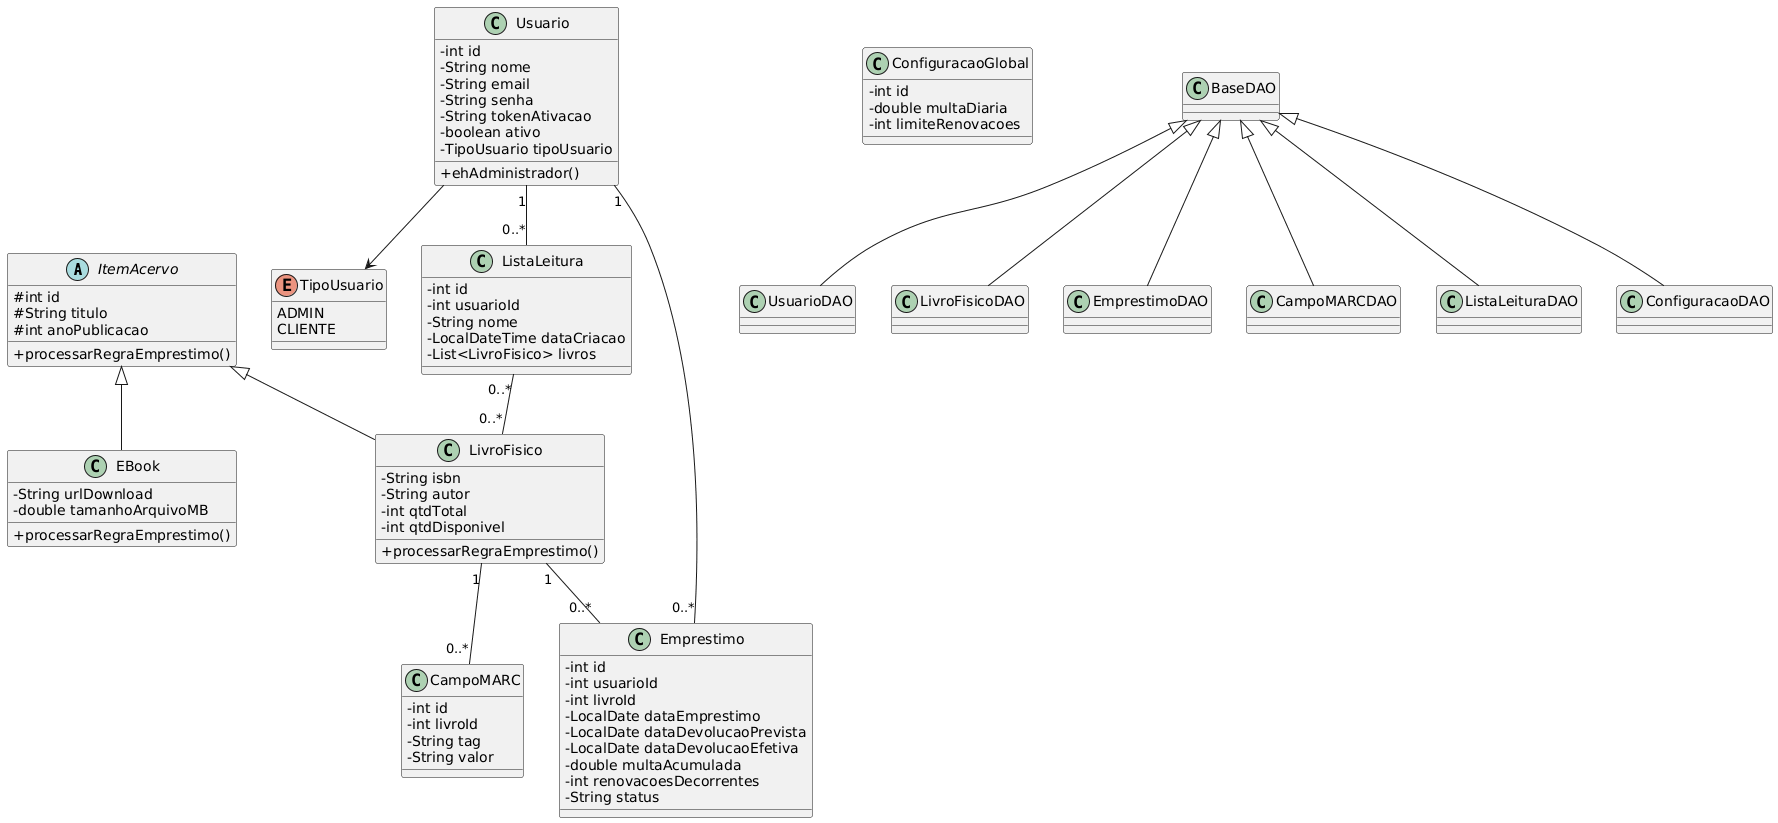
\includegraphics[width=\textwidth,height=0.72\textheight,keepaspectratio]{../imagens/1-class_diagram.png}
	\caption{Diagrama de Classes do sistema Biblioteca MARC21}
	\label{fig:diagrama-classes}
\end{figure}

As principais relações de herança e associação são:

\begin{itemize}
	\item \textbf{\texttt{ItemAcervo} (Abstrata)} $\leftarrow$ \texttt{LivroFisico}: Representa obras físicas do acervo com controle de quantidade disponível em estoque.
	\item \textbf{\texttt{ItemAcervo} (Abstrata)} $\leftarrow$ \texttt{EBook}: Representa livros digitais com URL de acesso e sem restrição de quantidade.
	\item \textbf{\texttt{BaseDAO} (Abstrata)} $\leftarrow$ Todos os DAOs: Centraliza a lógica de obtenção de conexão JDBC.
	\item \textbf{\texttt{Emprestimo}} associa \texttt{Usuario} e \texttt{LivroFisico}: Representa a solicitação e, após aprovação administrativa, o contrato de retirada física.
\end{itemize}

\subsection{Arquitetura de Fluxo de Dados}

O fluxo de execução das requisições assíncronas (AJAX) segue de forma padronizada o seguinte caminho:

\begin{center}
	\texttt{Navegador} $\xrightarrow{\text{HTTP Request}}$ \texttt{AutenticacaoFilter} $\rightarrow$ \texttt{XServlet} $\rightarrow$ \texttt{XServletDAO} $\rightarrow$ \texttt{MySQL} \\[0.3cm]
	\texttt{MySQL} $\xrightarrow{\text{ResultSet}}$ \texttt{XServletDAO} $\rightarrow$ \texttt{Gson.toJson()} $\xrightarrow{\text{JSON}}$ \texttt{jQuery/AJAX} $\rightarrow$ \texttt{DOM}
\end{center}

\subsection{Diagrama Entidade-Relacionamento}

O modelo relacional do banco de dados organiza os cadastros principais e as relações operacionais de empréstimo, metadados MARC21 e listas de leitura.

\begin{figure}[htbp]
	\centering
	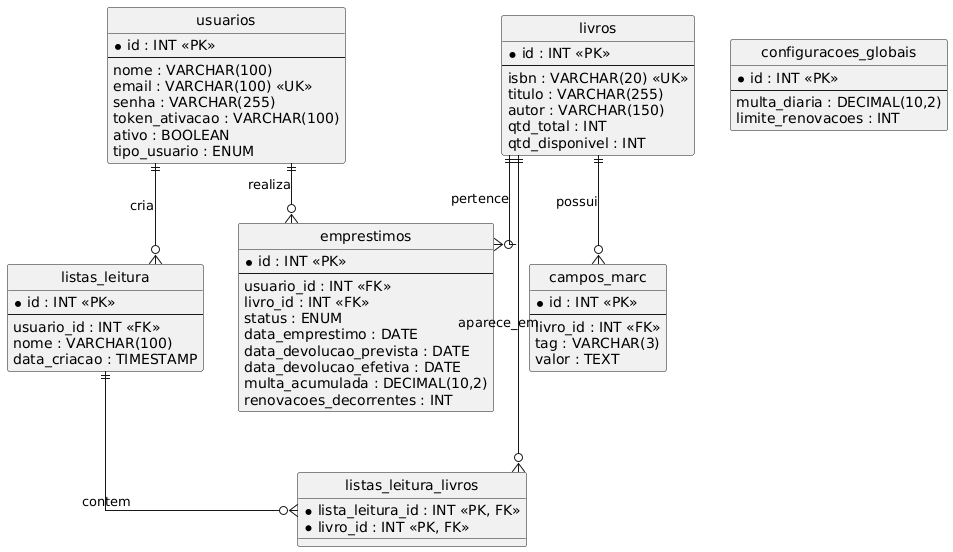
\includegraphics[width=\textwidth,height=0.72\textheight,keepaspectratio]{../imagens/2-entity_diagram.png}
	\caption{Diagrama Entidade-Relacionamento do banco de dados}
	\label{fig:diagrama-er}
\end{figure}

\subsection{Diagrama de Caso de Uso}

\begin{figure}[htbp]
	\centering
	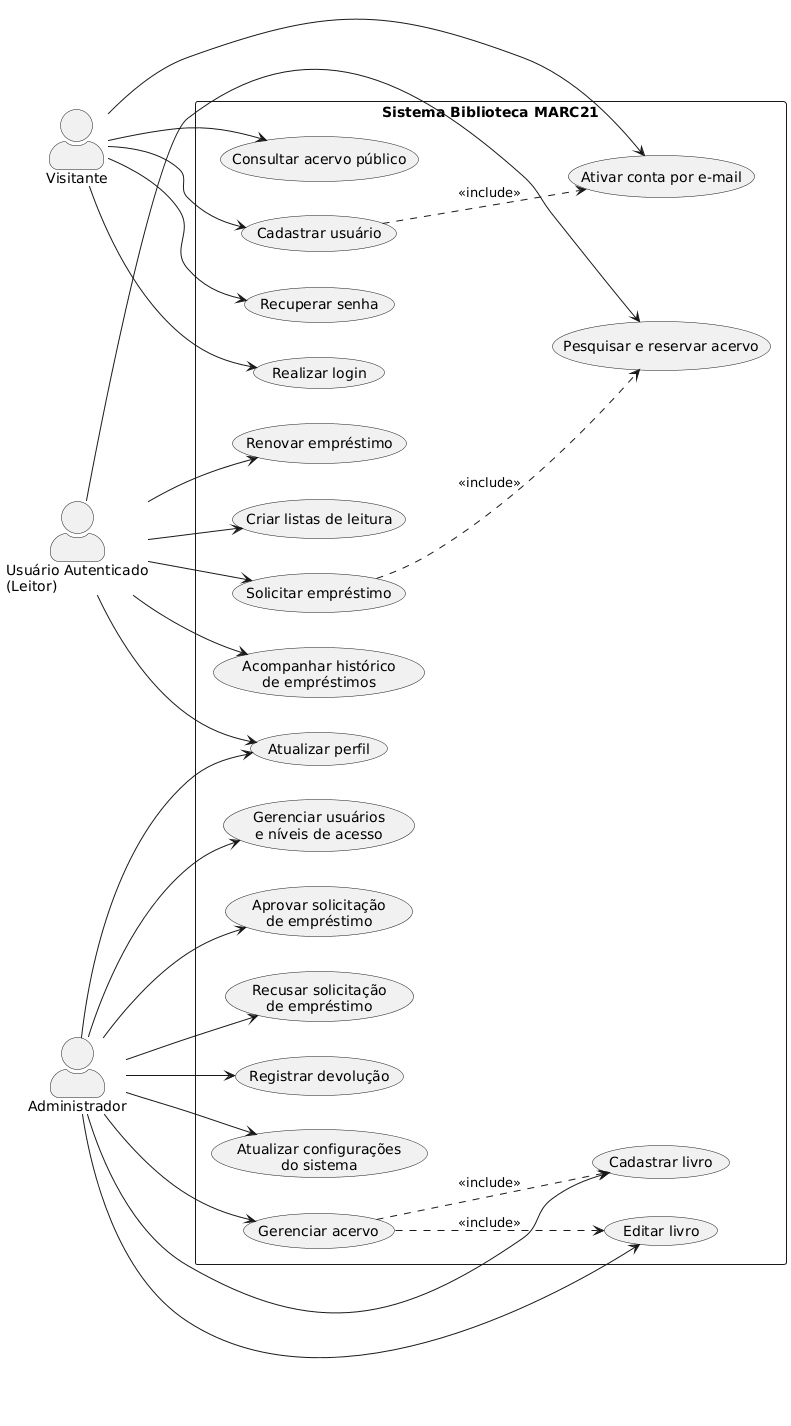
\includegraphics[width=\textwidth,height=0.72\textheight,keepaspectratio]{../imagens/3-use_case_diagram.png}
	\caption{Diagrama de Caso de Uso}
	\label{fig:diagrama-caso-uso}
\end{figure}

\subsection{Diagrama de Sequência: Solicitação e Aprovação de Empréstimo}

\begin{figure}[htbp]
	\centering
	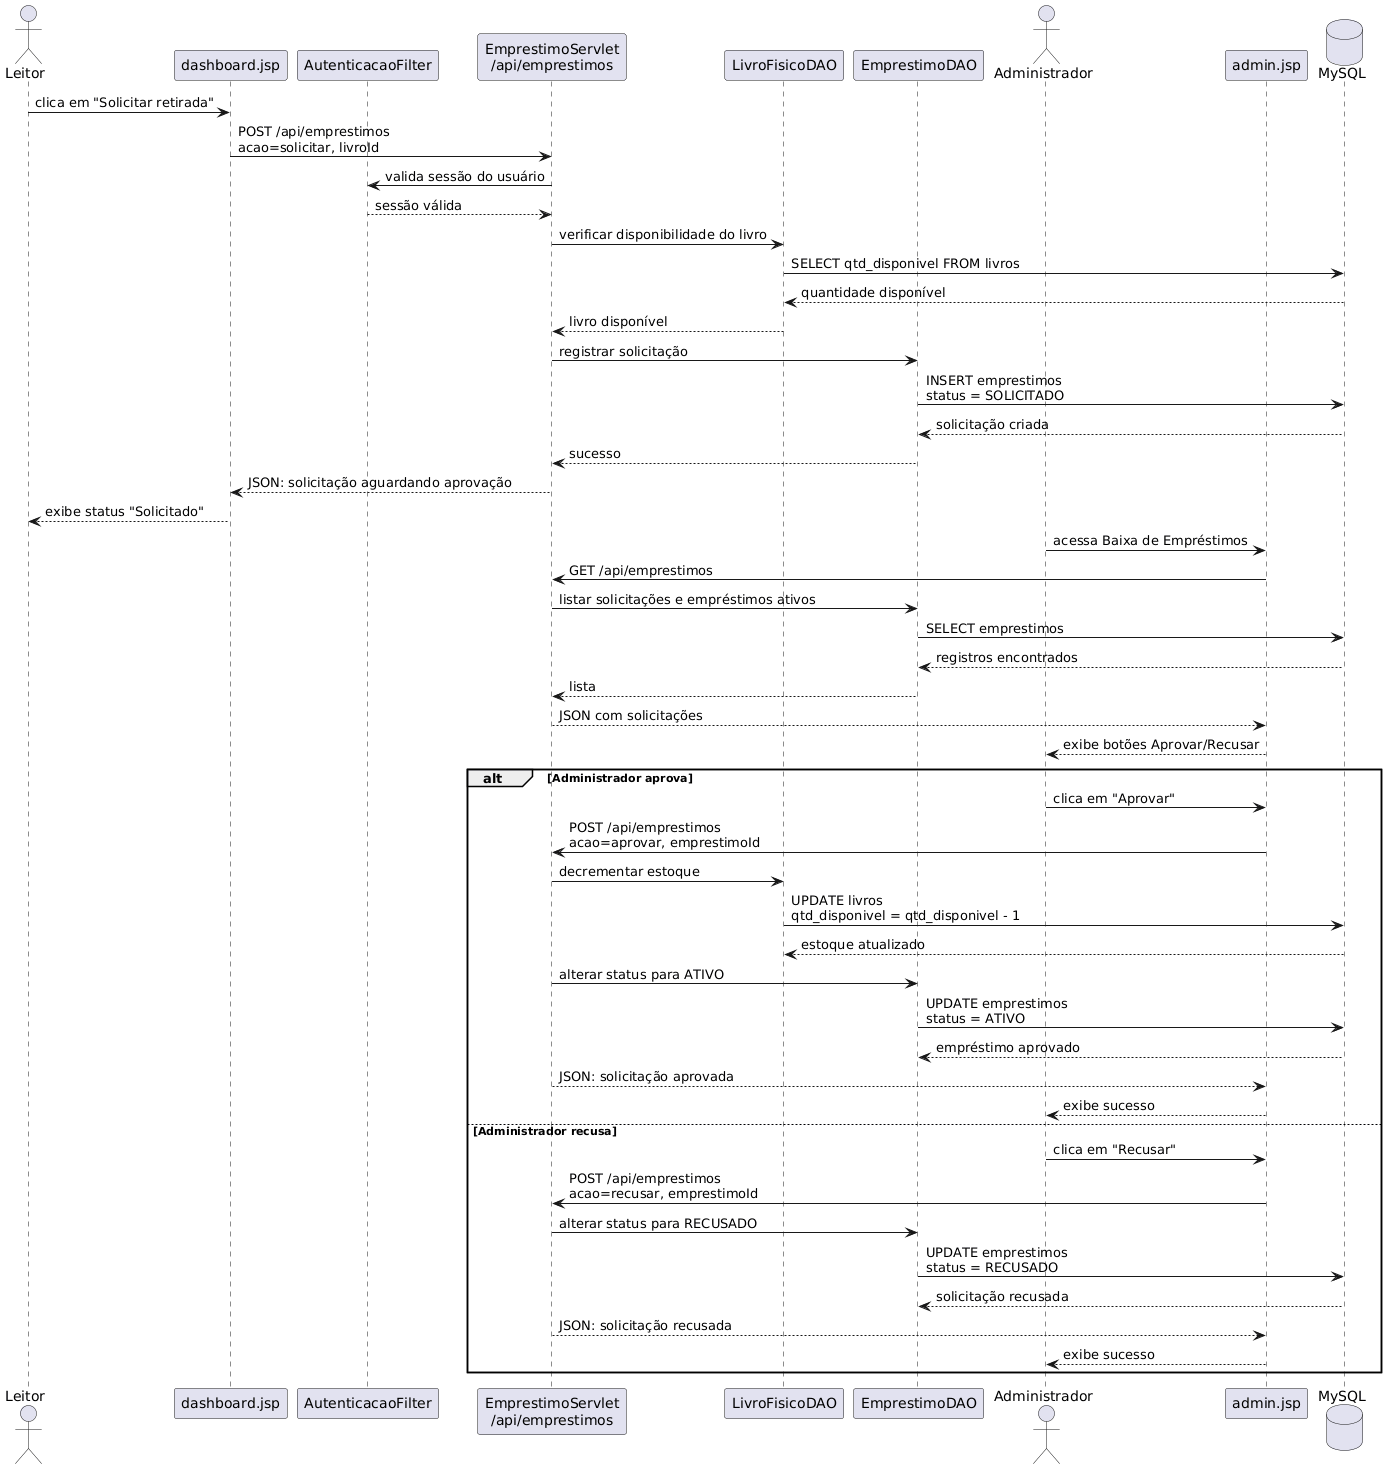
\includegraphics[width=\textwidth,height=0.72\textheight,keepaspectratio]{../imagens/4-sequence_diagram.png}
	\caption{Diagrama de Sequência: solicitação e aprovação de empréstimo}
	\label{fig:diagrama-sequencia-emprestimo}
\end{figure}

	
	\section{Relatório de Testes de Endpoints}
	\label{sec:testes_endpoints}

Os endpoints da aplicação foram testados utilizando a ferramenta \textbf{Postman} (versão 10+). Para cada endpoint, foram realizados testes com dados válidos e dados inválidos para verificar o comportamento esperado da API.

\textbf{Configuração do ambiente de teste:}
\begin{itemize}
	\item URL Base: \texttt{http://localhost:8080/biblioteca}
	\item Servidor: Apache Tomcat 9.0 (local)
	\item Banco de Dados: MySQL 8.0 (local)
\end{itemize}

% ---- ENDPOINT 1: POST /api/login ----
\subsection{Endpoint: POST /api/login}

\textbf{Descrição:} Autentica o usuário e retorna os dados da sessão em JSON.

\textbf{Teste 1.1 --- Login de Administrador com sucesso:}

\begin{lstlisting}[style=sqlStyle, caption={Requisição: POST /api/login (Administrador)}]
	POST http://localhost:8080/biblioteca/api/login
	Content-Type: application/x-www-form-urlencoded
	
	email=admin@biblioteca.com&senha=admin123
\end{lstlisting}

\begin{lstlisting}[style=sqlStyle, caption={Resposta esperada (HTTP 200 OK)}]
	{
		"sucesso": true,
		"mensagem": "Login realizado com sucesso.",
		"usuario": {
			"id": 1,
			"nome": "Administrador",
			"perfil": "ADMIN",
			"redirect": "/biblioteca/admin.jsp"
		}
	}
\end{lstlisting}

\textbf{Teste 1.2 --- Login com credenciais inválidas:}

\begin{lstlisting}[style=sqlStyle, caption={Resposta esperada (HTTP 401 Unauthorized)}]
	{
		"sucesso": false,
		"mensagem": "E-mail ou senha invalidos."
	}
\end{lstlisting}

% ---- ENDPOINT 2: POST /api/usuarios ----
\subsection{Endpoint: POST /api/usuarios}

\textbf{Descrição:} Realiza o cadastro de um novo leitor no sistema.

\begin{lstlisting}[style=sqlStyle, caption={Requisição: POST /api/usuarios}]
	POST http://localhost:8080/biblioteca/api/usuarios
	Content-Type: application/x-www-form-urlencoded
	
	nome=Fulano+da+Silva&email=fulano@gmail.com&senha=senha123
\end{lstlisting}

\begin{lstlisting}[style=sqlStyle, caption={Resposta esperada (HTTP 201 Created)}]
	{
		"sucesso": true,
		"mensagem": "Cadastro realizado com sucesso! Verifique seu e-mail para ativar a conta."
	}
\end{lstlisting}

\textbf{Teste 2.2 --- Tentativa de cadastro com e-mail duplicado:}

\begin{lstlisting}[style=sqlStyle, caption={Resposta esperada (HTTP 409 Conflict)}]
	{
		"sucesso": false,
		"mensagem": "Este e-mail ja esta cadastrado."
	}
\end{lstlisting}

% ---- ENDPOINT 3: GET /api/ativar ----
\subsection{Endpoint: GET /api/ativar}

\textbf{Descrição:} Ativa a conta do usuário através do token UUID enviado por e-mail.

\begin{lstlisting}[style=sqlStyle, caption={Requisição: GET /api/ativar}]
	GET http://localhost:8080/biblioteca/api/ativar?token=9b1deb4d-3b7d-4bad-9bdd-2b0d7b3dcb6d
\end{lstlisting}

\begin{lstlisting}[style=sqlStyle, caption={Resposta esperada (HTTP 200 OK)}]
	{
		"sucesso": true,
		"mensagem": "Conta ativada com sucesso! Voce ja pode fazer login."
	}
\end{lstlisting}

% ---- ENDPOINT 4: POST /api/recuperar ----
\subsection{Endpoint: POST /api/recuperar}

\textbf{Descrição:} Envia uma senha temporária por e-mail se a conta estiver ativa.

\begin{lstlisting}[style=sqlStyle, caption={Requisição: POST /api/recuperar}]
	POST http://localhost:8080/biblioteca/api/recuperar
	Content-Type: application/x-www-form-urlencoded
	
	email=fulano@gmail.com
\end{lstlisting}

\begin{lstlisting}[style=sqlStyle, caption={Resposta esperada (HTTP 200 OK)}]
	{
		"sucesso": true,
		"mensagem": "Se o e-mail existir e a conta estiver ativa, enviaremos uma senha temporaria."
	}
	\\end{lstlisting}
	
	% ---- ENDPOINT 5: POST /api/emprestimos ----
	\subsection{Endpoint: POST /api/emprestimos}
	
	\textbf{Descrição:} Registra uma solicitação de empréstimo para um livro físico disponível. O estoque somente é alterado depois da aprovação administrativa.
	
	\begin{lstlisting}[style=sqlStyle, caption={Requisição: POST /api/emprestimos}]
		POST http://localhost:8080/biblioteca/api/emprestimos
		Content-Type: application/x-www-form-urlencoded
		Cookie: JSESSIONID={token_da_sessao_leitor}
		
		acao=cadastrar\&livroId=5
	\end{lstlisting}
	
	\begin{lstlisting}[style=sqlStyle, caption={Resposta esperada (HTTP 200 OK)}]
		{
			"sucesso": true,
			"mensagem": "Solicitacao enviada com sucesso! Aguarde a aprovacao do administrador para retirar o livro."
		}
	\end{lstlisting}

	\textbf{Teste 5.1 --- Admin aprova solicitação de empréstimo:}

	\begin{lstlisting}[style=sqlStyle, caption={Requisição: POST /api/emprestimos acao=aprovar}]
		POST http://localhost:8080/biblioteca/api/emprestimos
		Content-Type: application/x-www-form-urlencoded
		Cookie: JSESSIONID={token_da_sessao_admin}
		
		acao=aprovar\&emprestimoId=10
	\end{lstlisting}

	\begin{lstlisting}[style=sqlStyle, caption={Resposta esperada (HTTP 200 OK)}]
		{
			"sucesso": true,
			"mensagem": "Solicitacao aprovada. O emprestimo foi iniciado..."
		}
	\end{lstlisting}

	\textbf{Teste 5.2 --- Admin recusa solicitação de empréstimo:}

	\begin{lstlisting}[style=sqlStyle, caption={Requisição: POST /api/emprestimos acao=recusar}]
		POST http://localhost:8080/biblioteca/api/emprestimos
		Content-Type: application/x-www-form-urlencoded
		Cookie: JSESSIONID={token_da_sessao_admin}
		
		acao=recusar\&emprestimoId=10
	\end{lstlisting}

	\begin{lstlisting}[style=sqlStyle, caption={Resposta esperada (HTTP 200 OK)}]
		{
			"sucesso": true,
			"mensagem": "Solicitacao recusada sem alterar o estoque."
		}
	\end{lstlisting}
	
	\textbf{Teste 5.3 --- Usuário não autenticado tentando acessar:}
	
	\begin{lstlisting}[style=sqlStyle, caption={Resposta esperada (HTTP 401 Unauthorized)}]
		{
			"sucesso": false,
			"mensagem": "Acesso negado. Faca login primeiro."
		}
	\end{lstlisting}
	
	\textbf{Teste 5.4 --- Leitor tentando acessar endpoint de Admin:}
	
	\begin{lstlisting}[style=sqlStyle, caption={Resposta esperada (HTTP 403 Forbidden)}]
		{
			"sucesso": false,
			"mensagem": "Acesso negado. Permissao insuficiente."
		}
	\end{lstlisting}
	
	\subsection{Endpoint: GET/POST /api/admin/usuarios}
	
	\textbf{Descrição:} Lista usuários cadastrados e permite ao administrador alterar perfil e status.
	
	\begin{lstlisting}[style=sqlStyle, caption={Requisição: POST /api/admin/usuarios}]
		POST http://localhost:8080/biblioteca/api/admin/usuarios
		Content-Type: application/x-www-form-urlencoded
		Cookie: JSESSIONID={token_da_sessao_admin}
		
		id=2\&tipoUsuario=CLIENTE\&ativo=true
	\end{lstlisting}
	
	\begin{lstlisting}[style=sqlStyle, caption={Resposta esperada (HTTP 200 OK)}]
		{
			"sucesso": true,
			"mensagem": "Usuario atualizado com sucesso."
		}
	\end{lstlisting}
	
	\subsection{Endpoint: GET/POST /api/admin/configuracoes}
	
	\textbf{Descrição:} Consulta e atualiza parâmetros operacionais do sistema.
	
	\begin{lstlisting}[style=sqlStyle, caption={Requisição: POST /api/admin/configuracoes}]
		POST http://localhost:8080/biblioteca/api/admin/configuracoes
		Content-Type: application/x-www-form-urlencoded
		Cookie: JSESSIONID={token_da_sessao_admin}
		
		multaDiaria=2.50\&limiteRenovacoes=3\&prazoEmprestimo=7
	\end{lstlisting}
	
	\begin{lstlisting}[style=sqlStyle, caption={Resposta esperada (HTTP 200 OK)}]
		{
			"sucesso": true,
			"mensagem": "Parametros operacionais atualizados com sucesso."
		}
	\end{lstlisting}

	
	\section{Relatório de Testes de Funcionalidades}
	Esta seção documenta os testes realizados nas funcionalidades completas do sistema,
verificando o fluxo de ponta a ponta (interface $\\rightarrow$ AJAX $\\rightarrow$ Servlet $\\rightarrow$ DAO $\\rightarrow$ MySQL).

% ---- FUNCIONALIDADE 1: CADASTRO E ATIVAÇÃO ----
\subsection{Funcionalidade: Cadastro e Ativação de Conta}

\textbf{Objetivo:} Verificar o fluxo completo de registro de um novo usuário, incluindo o
recebimento e validação do e-mail de ativação via Mailtrap.

\begin{table}[h!]
	\centering
	\caption{Casos de teste --- Cadastro e Ativação}
	\label{tab:teste_cadastro}
	\begin{tabular}{|c|p{6cm}|p{6cm}|c|}
		\hline
		\textbf{CT\#} & \textbf{Ação} & \textbf{Resultado Esperado} & \textbf{Status} \\ \hline
		CT-01 & Preencher todos os campos do formulário de cadastro com dados válidos e submeter. & Mensagem de sucesso exibida via AJAX; e-mail de ativação enviado ao Mailtrap. & $\checkmark$ \\ \hline
		CT-02 & Submeter o formulário com o campo e-mail em branco. & Validação HTML5/jQuery impede envio; mensagem de erro ``Campo obrigatório''. & $\checkmark$ \\ \hline
		CT-03 & Tentar cadastrar com um e-mail já existente no banco. & Retorno JSON com erro 409; mensagem ``E-mail já cadastrado'' exibida na tela. & $\checkmark$ \\ \hline
		CT-04 & Acessar o link de ativação recebido no Mailtrap. & Conta ativada; redirecionamento para login com mensagem de confirmação. & $\checkmark$ \\ \hline
	\end{tabular}
\end{table}

% ---- FUNCIONALIDADE 2: AUTENTICAÇÃO ----
\subsection{Funcionalidade: Autenticação e Controle de Acesso}

\begin{table}[h!]
	\centering
	\caption{Casos de teste --- Login e RBAC}
	\label{tab:teste_login}
	\begin{tabular}{|c|p{6cm}|p{6cm}|c|}
		\hline
		\textbf{CT\#} & \textbf{Ação} & \textbf{Resultado Esperado} & \textbf{Status} \\ \hline
		CT-05 & Efetuar login com credenciais de Administrador. & Usuário autenticado com sucesso e redirecionado para \texttt{admin.jsp}. & $\checkmark$ \\ \hline
		CT-06 & Efetuar login com credenciais de Leitor (ativo). & Usuário autenticado com sucesso e redirecionado para \texttt{dashboard.jsp}. & $\checkmark$ \\ \hline
		CT-07 & Tentar logar com conta existente mas não ativada por e-mail. & Mensagem informando a necessidade de validação de conta antes do primeiro acesso. & $\checkmark$ \\ \hline
		CT-08 & Inserir senha incorreta para e-mail cadastrado. & Erro capturado; mensagem ``E-mail ou senha inválidos'' sem expor detalhes estruturais. & $\checkmark$ \\ \hline
		CT-09 & Leitor tenta digitar diretamente a URL \texttt{/admin.jsp}. & Bloqueado por \texttt{AutenticacaoFilter} e redirecionado ao index com aviso de restrição. & $\checkmark$ \\ \hline
	\end{tabular}
\end{table}

% ---- FUNCIONALIDADE 3: CATALOGAÇÃO ----
\subsection{Funcionalidade: Catalogação e Filtros do Acervo (MARC21)}

\begin{table}[h!]
	\centering
	\caption{Casos de teste --- Acervo e MARC21}
	\label{tab:teste_acervo}
	\begin{tabular}{|c|p{6cm}|p{6cm}|c|}
		\hline
		\textbf{CT\#} & \textbf{Ação} & \textbf{Resultado Esperado} & \textbf{Status} \\ \hline
		CT-10 & Admin insere um livro físico mapeando as tags MARC21 (020, 100, 245). & Dados distribuídos corretamente entre as tabelas correspondentes no MySQL. & $\checkmark$ \\ \hline
		CT-11 & Admin tenta cadastrar item sem preencher a Tag 245 (Título obrigatório). & Alerta de validação impede o envio; transação não enviada ao banco de dados. & $\checkmark$ \\ \hline
		CT-12 & Usuário realiza busca rápida por termo presente na tag de assunto (Tag 650). & Listagem atualizada dinamicamente via AJAX exibindo apenas os registros correspondentes. & $\checkmark$ \\ \hline
		CT-13 & Leitor clica em visualizar detalhes de uma obra física do acervo. & Modal abre exibindo a ficha catalográfica formatada com os rótulos legíveis das Tags MARC21. & $\checkmark$ \\ \hline
	\end{tabular}
\end{table}

% ---- FUNCIONALIDADE 4: EMPRÉSTIMOS ----
\subsection{Funcionalidade: Controle de Empréstimos e Devoluções}

\begin{table}[h!]
	\centering
	\caption{Casos de teste --- Empréstimos}
	\label{tab:teste_emprestimos}
	\begin{tabular}{|c|p{6cm}|p{6cm}|c|}
		\hline
		\textbf{CT\#} & \textbf{Ação} & \textbf{Resultado Esperado} & \textbf{Status} \\ \hline
		CT-14 & Leitor solicita empréstimo de livro com estoque disponível. & Registro criado com status \texttt{SOLICITADO}; estoque permanece inalterado até aprovação administrativa. & $\checkmark$ \\ \hline
		CT-15 & Leitor tenta solicitar livro que está com estoque zerado (indisponível). & Botão desabilitado na interface; requisição manual direta via endpoint devolve erro. & $\checkmark$ \\ \hline
		CT-16 & Admin aprova uma solicitação pendente. & Status alterado para \texttt{ATIVO}; data de retirada atualizada; estoque decrementado em 1 unidade. & $\checkmark$ \\ \hline
		CT-17 & Admin recusa uma solicitação pendente. & Status alterado para \texttt{RECUSADO}; estoque permanece inalterado. & $\checkmark$ \\ \hline
		CT-18 & Admin registra devolução dentro do prazo regulamentar. & Status do empréstimo alterado para \texttt{DEVOLVIDO}; estoque incrementado em +1 unidade. & $\checkmark$ \\ \hline
		CT-19 & Admin registra devolução de empréstimo com 3 dias de atraso. & Sistema calcula automaticamente o valor da multa com base na taxa diária operacional vigente. & $\checkmark$ \\ \hline
	\end{tabular}
\end{table}

% ---- FUNCIONALIDADE 5: RENOVAÇÃO ----
\subsection{Funcionalidade: Renovação Online e Regras de Negócio}

\begin{table}[h!]
	\centering
	\caption{Casos de teste --- Renovações}
	\label{tab:teste_renovacao}
	\begin{tabular}{|c|p{6cm}|p{6cm}|c|}
		\hline
		\textbf{CT\#} & \textbf{Ação} & \textbf{Resultado Esperado} & \textbf{Status} \\ \hline
		CT-20 & Leitor solicita renovação de empréstimo ativo dentro do prazo regular. & Data de devolução estendida por mais 7 dias; contador incrementado. & $\checkmark$ \\ \hline
		CT-21 & Leitor tenta renovar uma solicitação ainda não aprovada. & Renovação recusada; apenas empréstimos com status \texttt{ATIVO} podem ser renovados. & $\checkmark$ \\ \hline
		CT-22 & Leitor tenta renovar um empréstimo já em atraso (vencido). & Renovação recusada; sistema exige a devolução imediata do item físico e quitação do débito. & $\checkmark$ \\ \hline
		CT-23 & Leitor tenta realizar a 4ª renovação consecutiva (limite configurado = 3). & Ação bloqueada pelo servidor; mensagem de erro indica limite de renovações atingido. & $\checkmark$ \\ \hline
	\end{tabular}
\end{table}

% ---- FUNCIONALIDADE 6: CONFIGURAÇÕES ----
\subsection{Funcionalidade: Configurações do Sistema}

\begin{table}[h!]
	\centering
	\caption{Casos de teste --- Configurações}
	\label{tab:teste_config}
	\begin{tabular}{|c|p{6cm}|p{6cm}|c|}
		\hline
		\textbf{CT\#} & \textbf{Ação} & \textbf{Resultado Esperado} & \textbf{Status} \\ \hline
		CT-24 & Admin altera o valor da multa diária para R\$ 2,50. & Novo valor persistido no banco; próximo cálculo de multa usa o valor atualizado. & $\checkmark$ \\ \hline
		CT-25 & Admin altera o limite de renovações para 1 (mínimo). & Leitores que já renovaram uma vez não podem renovar novamente. & $\checkmark$ \\ \hline
		CT-26 & Leitor tenta acessar \texttt{GET /api/admin/configuracoes}. & HTTP 403 retornado pelo \texttt{AutenticacaoFilter}. & $\checkmark$ \\ \hline
	\end{tabular}
\end{table}

% ---- FUNCIONALIDADE 7: USUÁRIOS ----
\subsection{Funcionalidade: Perfil e Controle de Usuários}

\begin{table}[h!]
	\centering
	\caption{Casos de teste --- Perfil e Usuários}
	\label{tab:teste_usuarios}
	\begin{tabular}{|c|p{6cm}|p{6cm}|c|}
		\hline
		\textbf{CT\#} & \textbf{Ação} & \textbf{Resultado Esperado} & \textbf{Status} \\ \hline
		CT-27 & Leitor atualiza nome e senha no painel. & Dados persistidos; sessão atualizada; senha gravada com hash SHA-256. & $\checkmark$ \\ \hline
		CT-28 & Admin altera papel de usuário de 'Leitor' para 'Admin'. & Permissões atualizadas instantaneamente no banco de dados. & $\checkmark$ \\ \hline
		CT-29 & Admin inativa um usuário inadimplente crônico. & Usuário não consegue realizar login e tem acessos cortados. & $\checkmark$ \\ \hline
	\end{tabular}
\end{table}

	
	% ---------------------------------------------------------------------------
	% REFERÊNCIAS BIBLIOGRÁFICAS
	% ---------------------------------------------------------------------------
\newpage
\bibliographystyle{abbrv}
\nocite{*} % Força a exibição de todas as referências do .bib
\bibliography{../referencias}
	
\end{document}